\documentclass{article}
\usepackage{graphicx} % Required for inserting images
\usepackage[
backend=biber,
style=numeric,
sorting=ynt
]{biblatex}
\addbibresource{sources.bib}
\usepackage{booktabs}
\usepackage{amsmath}
\usepackage{multirow}
\usepackage{hyperref}
\graphicspath{ {./images/} }

\begin{document}

\begin{titlepage}

    \begin{center}
        \large
        National Research University Higher School of Economics\\
        Faculty of Computer Science\\
        Programme ‘Master of Data Science’

        \vspace{2cm}
        MASTER'S THESIS\\
        topic\\
        \Huge
        \textbf{Application of Machine Learning for Early Crop Classification Using Satellite Imagery}
    \end{center}
    
    \vspace{1cm}
    \Large
    \textbf{Student:} Syomin Pavel Olegovich

    \vspace{2cm}
    \Large
    \textbf{Supervisor:} Maksimovskaya Anastasia Maksimovna
    
    \vfill

    \begin{center}
        \large
        Moscow, 2023
    \end{center}      
    
\end{titlepage}

\thispagestyle{plain}
\begin{center}
    \Large
    \textbf{Application of Machine Learning for Early Crop Classification Using Satellite Imagery}
    
    \vspace{0.4cm}
    \textbf{Pavel O. Syomin}
    
    \vspace{0.9cm}
    \textbf{Abstract}
\end{center}

In this thesis, the problem of early crop classification is being solved. Typically crop classification is performed using time series of satellite shots that cover the whole vegetation season. Early classification is a prediction of a crop cultivated on a field using the shortest possible time series counting from the beginning of the season. In this study, a private ground-truth dataset of Russian fields for 2018–2022 is used, as well as an open collection of Sentinel-2 satellite images. Two approaches for early classification are compared, the first is the ensembles of generic models trained on varying-length input time series, and the second is special models optimized jointly for accuracy and earliness. Both classical tree-based machine learning methods (namely, Random Forest, LightGBM, and CatBoost) and novel deep learning methods (namely, recurrent, convolutional and attention-based neural networks) are applied. Also, an original EarlyTempCNN model combining a convolutional backbone with two heads and simultaneous optimization for earliness and accuracy is proposed. It is found that there is an opportunity to classify crops utilizing only $2/3$ of full-length time series with an insignificant reduction in quality or even without any loss in scores, if the models have been trained on a large enough dataset. Special models with joint optimization show top scores on the small dataset, but on the larger dataset, their performance is on the level of tree-based baseline solutions. However, such models provide for additional benefits like reduced training time compared to the ensembles, higher interpretability resulting from confidence estimates and probability distributions for each timestamp, individualization of predictions so that the decision for each field is made separately, and overall opportunity for building real-time fine-tuned solutions. The proposed EarlyTempCNN model has achieved one of the best scores on the small dataset, but on the large dataset, its performance has decreased.



\newpage

\tableofcontents
\newpage

\section{Introduction}

\subsection{Motivation and Significance of the Topic}
This research started as a part of my job project on crop classification using satellite remote sensing data. While conducting its operations, the company has collected a substantial amount of ground-truth information about crops cultivated on fields in various regions of Russia. The overall idea was to use this information to train a model predicting crops based on remote sensing data. The predictions of the model may have been used for various business applications, including statistics or control services, marketing, and new tools for agricultural companies. Eventually, the desired model was made, but questions about further improvement of this model have arisen.

Crop classification is usually made by analysis of time series of satellite shots. For accurate predictions, the long time series spreading for the whole season from spring to autumn are required. Here and later, I will call them a “full-length” time series. The processing of the large number of satellite shots is expensive both in terms of computations and storage. For production use, it is better to reduce the amount of data required for accurate classification. Also, the need to use the whole season means that, in the general case, only historical datasets for the previous years may be used, and the prediction for the current season is impossible, thus limiting the range of potential business applications of the model.

Consequently, the problem arises: how can one correctly classify crops using time series which cover just a part of the season? In other words, can we use a shorter sequence of satellite images while preserving the sufficient quality of the model? I dived into this problem, and it became both my job duty and a research project for a Master's thesis.

\subsection{Related Works}

Crop classification with machine learning is quite a well-researched set of tasks with many theoretical approaches, technologies available, and potential practical applications. In general, we can list several groups of methods and ways of solving this problem.

Based on the data available, there is a crop classification with multispectral or hyperspectral shots, where multispectral shots have wider bands (10–100 nm) and a smaller number of channels (about 10) compared to hyperspectral shots with very narrow bands (up to a few nanometers) and a great number of channels (up to a hundred). For example, in \cite{agronomy9090496} the authors focus on creating the collection of crop-specific hyperspectral features that can be used for the classification. On the contrary, in \cite{7891032}, multispectral shots are used.

Remote sensing data may be either airborne (that is, collected using unmanned aerial vehicles), like in \cite{app9040643}, or satellite. Satellite data is, in general, easier to obtain because there are open collections of space images, and it has nearly global coverage but it also suffers from a number of disadvantages, including lower temporal, spatial, and spectral resolution, cloud cover, and atmospheric distortions. In contrast, airborne data is usually of better resolution, but is harder to obtain because of the need to launch a drone, and the spatial coverage is relatively small.

Another division of data types is optical and radiometric data. It means that shots may be made either in a visual specter (or close to it) or in the microwaves specter. It is stated that radiometric data is not sensitive to weather conditions because clouds are transparent to microwaves, and thus sometimes it is a preferred choice \cite{DANDRIMONT2021112708}. Radiometric data may be used in combination with optical data \cite{Moumni2021}.

The number of shots used for crop classification may be different. A more usual approach is to get a time series of images \cite{7891032, DANDRIMONT2021112708, Moumni2021, ZHONG2019430}. The length of this series may range from a part of the season \cite{rußwurm2022endtoend} to several seasons \cite{quinton2021crop}. A less common, but also applicable way to predict crops is a single-shot classification \cite{MENG2021106188}.

The problem of crop classification may be seen from two points of view, and as a result, two group of methods exist. The first can be called parcel-based, and the second can be named pixel-based \cite{doi:10.5721/EuJRS20124535}. Applying the parcel-based approach, a user extracts features of a given land parcel and feeds them into a model. For example, this method is used in \cite{brandt2019spatiotemporal}. In the pixel-based approach, a model receives the whole image (or a sequence of images) as an input and produces a map of labels for each pixel or detects objects of given types. For example, in \cite{WANG2022107249}, the authors processed space shots as regular images and applied a UNet++ model for semantic segmentation. Parcel-based approach is a classification task (and it usually belongs to a subcategory of time series classification), while pixel-based approach is an image segmentation or object detection task. Consequently, the models applied in these groups of methods are also different. In \cite{doi:10.5721/EuJRS20124535}, pixel-based and parcel-based methods are compared, and parcel-based methods show better scores.

Crop classification task can be solved by classical machine learning models, by deep learning models, or by ensembles of models. In 2000s and at the beginning of 2010s classical models were common (e.g. they are used in \cite{doi:10.5721/EuJRS20124535}), but now deep learning models generally outperform classical approaches. So, neural networks today can be considered a state-of-the-art technique, while traditional methods often act as a baseline (this is obvious, for example, in \cite{breizhcrops2020}). Among classical models, random forest, support vector machines and various tree-based boosting algorithms like XGBoost are used \cite{ZHONG2019430}. As for deep learning models, the popular choices are recurrent and convolutional neural networks, transformers, and several image segmentation models like UNet or DeepLabv3+ \cite{WANG2022107249}.

The solutions to the problem of crop classification have advanced through years, and models have reached quite good performance. As a result, the vanilla problem of classification has become less interesting for researchers, and they have moved their focus on several subproblems and side tasks. Examples of such subproblems and tasks are a creation of datasets and benchmarks for crop classification \cite{breizhcrops2020, sykas2022sentinel2}, spatial and temporal generalization of models \cite{nyborg2022generalized, khanna2022activation}, overcoming the issue of missing observations resulted from cloud cover \cite{metzger2021crop}, and early classification \cite{rußwurm2022endtoend} which is the main objective of this thesis.

\subsection{Problem Statement}

There is ground-truth data on crops cultivated on a few thousand fields in various regions of Russia for 2018–2022. There is also an open collection of satellite shots that covers the required period. For each field and for each year, a time series of satellite shots can be constructed which starts in April and ends in September. Given this time series, the goal is to correctly predict the crop on the field using as short a time series as possible counting the length of the time series from the beginning of the season, i.e. from April.

As mentioned in “Related Works” subsection, there are many possible ways to solve this problem. With respect to various limitations, the following approaches have been chosen. First, multispectral shots are used, because they are free of charge and publicly available, while hyperspectral imagery is commercial. The remote sensing data is satellite rather than airborne due to the large spatial extent of the area of interest and to the financial issues as well. Optical data is used to solve the task because it is easier to collect and process and because such an approach is more popular. A time series of shots are used because the results of single-shot classification with multispectral images known from related papers are often poor. A parcel-based approach is selected because it is less computationally expensive. Both classical and deep learning methods are used. The problem itself can be described as an early classification task which has already been investigated in some research papers.

\section{Dataset}

\subsection{Data Sources}

Ground truth data was provided by the company I am working for. It originated as a side result of the company's usual operations. The contours of fields, as well as information about crops cultivated on each field during each year, is provided to the company by individual farmers or agricultural organizations who are connected to the company's information system. This data is stored in a relational database. It was extracted from the database at the end of 2022 as a complete list of field unique identifiers, crop names for each year, and field contours.

As for remote sensing data, space shots from Sentinel-2 satellite were used. Sentinel-2 is a constellation of two Earth observation satellites launched by European Space Agency (ESA). It has nearly global coverage, and for the area of interest, the revisit time is 2–3 days. Sentinel-2 is a multispectral satellite with 13 bands. Subsequently, each shot is an image with 13 channels. Each shot covers an area of 110 × 110 sq. km. The spatial resolution of each shot varies from 10 to 60 meters depending on the channel. The space shots are available for the period from 2017 to now. The collection of Sentinel-2 images is open and free of charge. For this project, the collection of Sentinel-2 Cloud-Optimized GeoTIFFs on Amazon open data service was used (\url{https://registry.opendata.aws/sentinel-2-l2a-cogs/}). Raw Sentinel-2 data has already been preprocessed and atmospherically corrected by the ESA. For an end user, it looks as a set of multi-channel georeferenced GeoTIFF images which can be downloaded and applied in various tasks without additional preparations.

\subsection{Data Preparation Pipeline}

Data collection and preprocessing includes the following steps.

\begin{enumerate}
    \item Field ids, crop labels, and field contours are extracted from the company's database and stored in relevant formats. Also, the grid of expected shots contours is downloaded from Sentinel-2 website.
    \item Field contours are intersected with expected shots contours. Shots with a high number of fields are included in the downloads list, and shots with a small number of fields are not. The purpose of this step is to decrease the amount of downloaded data.
    \item Sentinel-2 satellite shots with processing level 2A (which means georeferencing and atmospheric correction) are downloaded from Sentinel-2 Cloud-Optimized GeoTIFFs open data archive on Amazon Web Services (see link above) according to the downloads list created on step 2 and saved in the cloud storage. Each shot has its timestamp, thus a collection of shots forms a time series.
    \item Using field contours from step 1, the respective parts of shots are cut and stored separately. If there is a field which does not fit into the single shot (e.g. it is on the border of two shots), a corresponding part is extracted from every shot and stored.
    \item From each part, the pixels with clouds or without data are removed.
    \item For each part, the median value of pixels for each channel is calculated.
    \item Values obtained on step 6 are combined and aggregated so that for each field and for each timestamp we have the median values of each of 13 bands.
    \item Three bands out of 13 (namely, 01, 09, and 10) are excluded from the dataset because their spatial resolution is low (60m).
    \item Spatial data is joined with ground-truth data (crop labels) by field id.
    \item The result is split into train and test parts (test size is 0.2) using a stratified split algorithm (for preserving proportions of classes). Train and test parts for each year are stored separately in CSV files.
\end{enumerate}

The length of time series for each field is different because of some properties of the data source and some aspects of the preprocessing pipeline. For example, the different revisit intervals for different geographical areas result in unequal time steps between consecutive elements of the series, and with the fixed length of the season, this inevitably leads to unequal time series length. Another reason for the differences is cloud cover: if a field for a given timestamp is covered with clouds, the corresponding time point is excluded from the dataset. Different length of sequences is an undesirable issue that may cause problems during training, so the time series for each field are linearly interpolated up to a fixed length of 182 (the number of days in a season). This interpolation is made at runtime.

\subsection{Dataset Description and Statistics}

The dataset is available for five years from 2018 to 2022. For the experiments, only 2018 year is used to minimize the amount of data, because the computational resources are limited. It contains 8624 observations in the train part and 2057 observations in the test part. Each observation represents a single field. An observation for a single field is a matrix of median values of each of 10 bands for each timestamp and a crop class label.

Crop labels, corresponding crop names, counts, and proportions of each class both in train and test parts of the dataset are shown in Table \ref{Table 2.3.1}.


\begin{table}
\centering
\caption{Crop Classes Statistics in the Dataset}
\label{Table 2.3.1}
\begin{tabular}{rlrrrr}
\toprule
 Class label &      Crop name &  \# in train &  \% in train &  \# in test &  \% in test \\
\midrule
           0 &           Corn &         590 &        7.14 &        147 &       7.15 \\
           1 &            Soy &         207 &        2.50 &         51 &       2.48 \\
           2 &      Sunflower &         635 &        7.68 &        158 &       7.68 \\
           3 &         Potato &          68 &        0.82 &         16 &       0.78 \\
           4 &      Sugarbeet &         182 &        2.20 &         45 &       2.19 \\
           5 &    Winter rape &          40 &        0.48 &          9 &       0.44 \\
           6 &    Spring rape &         425 &        5.14 &        106 &       5.15 \\
           8 & Winter cereals &        2379 &       28.79 &        594 &      28.88 \\
           9 & Spring cereals &        1442 &       17.45 &        360 &      17.50 \\
          10 &           Feed &         839 &       10.15 &        209 &      10.16 \\
          11 &         Fallow &         708 &        8.57 &        176 &       8.56 \\
          12 &          Other &         749 &        9.06 &        186 &       9.04 \\
\bottomrule
\end{tabular}
\end{table}

\subsection{Implementation Details}

For the experiments, the dataset is implemented as a Pytorch dataset. To work both with classical machine learning methods and neural networks, additional indexing by strings “X” and “y” returning the whole matrix of features or the whole array of labels is introduced. To accelerate the data interpolation which results are shared between experiments, a simple file-based caching is implemented. To support variable-length input sequences which are necessary for the experiments (see below), parameters to control the desired length of time series at runtime are provided. The full code of the dataset class is available in the thesis repository (see the link in the next section).

\section{Experimental Setup}

\subsection{General Approach}

As it has been previously described, the input data for each field is represented as a matrix of shape $T \times D$, where $T$ is the length of input time series, $D$ is the number of channels (bands), and the values are medians of surface reflectance in the given band for the given timestamp of all pixels within the borders of the field. In our experiments, $D$ is always 10 because we use 10 bands, but $T$ varies. An example of the matrix is shown below.

\[
\begin{bmatrix}

0.31 & 0.23 & 0.50 & 0.75 & 0.67 & 0.11 & 0.96 & 0.46 & 0.84 & 0.23 \\
1.00 & 0.75 & 0.90 & 0.34 & 0.65 & 0.45 & 0.20 & 0.19 & 0.76 & 0.15 \\
\vdots & \vdots & \vdots & \vdots & \vdots & \vdots & \vdots & \vdots & \vdots & \vdots \\
0.90 & 0.53 & 0.89 & 0.67 & 0.35 & 0.25 & 0.03 & 0.70 & 0.14 & 0.70

\end{bmatrix}_{T \times D}
\]

The goal is to train a model so that it will predict the crop label using as short a time series as possible. This can be achieved in two ways. The first way is to feed the model with subsamples of data having different length and thus representing a different time period from the beginning of the season. For example, if the length of the full season is 183 days, we can make subsamples of length $10, 20 , \ldots, 183$ days and train a separate model on each set of subsamples. In fact, the final estimator here is going to be an ensemble of models of the same type but trained on different datasets. The second way is to use a model which takes a full-length input, but is specially designed to predict the label using the shortest possible sequence. These two ways are compared in this research.

To sum it up, the plan for the experiments has two branches.

\begin{enumerate}
    \item Define a set of $T$ values. For each $T$ value, prepare a dataset limiting the length of input sequence by $T$. Take a “generic” model (i.e. a model which is not specifically tailored to early classification). On each dataset, train this model. Compare the performance of trained models to find out whether and how the length of input time series influences the performance. For inference, adjust the input length to the closest $T$ value and feed it into a relevant model from the pretrained set.
    \item Prepare a single dataset with full-length time series. Train a special model which tries to make a classification as early as possible. Look at the earliness of the classification and at the performance of the model to estimate whether and how the optimization for earliness influences the performance. For inference, use the pretrained model without extra preparations.
\end{enumerate}

\subsection{Models}

For the experiments, I use a few machine learning models of different types. Both classical tree-based models and deep learning neural networks are used. Also, the choice of the models depends on the experimental branch (see above), because to optimize simultaneously for earliness and accuracy, a special model is necessary.

Among classical machine learning models, I have selected Random Forest (RF) classifier, LightGBM classifier, and CatBoost classifier. All these models are tree-based ensembles. LightGBM and Catboost use gradient boosting to train “weak” trees on the residuals of the existing set of trees, while Random Forest trains a number of independent trees and averages their predictions. All these three models are trained on datasets with changing $T$, thus they belong to the first branch of the experiments.

As for neural networks, I have selected Transformer and TempCNN models. These models may have different architectures. I here rely on the models described in BreizhCrops paper \cite{breizhcrops2020}. Like tree-based models, both Transformer and TempCNN are trained on different datasets with changing $T$, thus they also belong to the first branch of the experiments.

For the joint optimization on earliness and accuracy, I use EarlyRNN and EarlyTempCNN models. EarlyRNN model was introduced in \cite{rußwurm2022endtoend}. It was specially designed to make as early a classification as possible while preserving comparable accuracy. Its architecture consists of three parts: backbone, classification head, and decision head. The backbone converts variable-length input time series into a fixed-size tensor of features. The classification head predicts a class label. The decision head predicts the probability of stopping, that is, it tries to decide whether the model has received enough data to infer a correct class label or it still has to obtain more data. A simultaneous optimization on earliness and accuracy is made by applying a specially designed loss function that combines classification loss with reward for earliness and by this tries to find the best trade-off between accuracy and speed. EarlyRNN in its original implementation uses a two-layers LSTM backbone. The backbone may be replaced by any other feature extractor compatible with classification and decision heads, thus I have made up my mind to build my own modification of EarlyRNN by replacing the original LSTM backbone with a convolutional backbone derived from TempCNN model. I have called the resulting model EarlyTempCNN.

To sum it up, in Table \ref{Table 3.2.1} there is a full list of models used during the experiments with additional information on the branch of experiments and models source.

\begin{table}
\centering
\caption{Models and Experiments}
\label{Table 3.2.1}
\begin{tabular}{l|l|c}
\toprule
Model name & Experiment branch & Source \\
\midrule
Random Forest & \multirow{5}{5cm}{\parbox{5cm}{\#1 (ensemble of models \\ built on datasets with different $T$)}} & \cite{ho1995random} \\
LightGBM  & & \cite{10.5555/3294996.3295074} \\
CatBoost & & \cite{dorogush2018catboost} \\
Transformer & & \cite{breizhcrops2020} \\
TempCNN & & \cite{breizhcrops2020} \\
\hline
EarlyRNN & \multirow{2}{5cm}{\parbox{5cm}{ \#2 (joint optimization \\ for earliness and accuracy)}} & \cite{rußwurm2022endtoend} \\
EarlyTempCNN & & Own \\
\bottomrule
\end{tabular}
\end{table}

\subsection{Scoring}

Due to a high class imbalance which is apparent from Table \ref{Table 2.3.1}, accuracy seems to be a mediocre metric of model performance. To overcome this issue, I have decided to use additional metrics: precision, recall, F1 score and kappa score. Among them, F1 score looks the most suitable, so it is by default reported in the results section.

\subsection{Implementation Details}

\begin{enumerate}
    \item  It looks that the most natural way to choose a set of $T$ is to make a split at the end of each month of the season. So, the first $T$ in the set corresponds to the end of April, the second — to the end of May, and so on. Consequently, the first dataset covers only April, the second is related to both April and May, and so on. The last dataset contains a full-length time series from the beginning of April to the end of September. If it is assumed that a month contains 30 days, then $T = \{30, 60, 90, 120, 150, 180\}$ (in fact, we have 183 days, but let us round them for the sake of simplicity). Here, $T = 30$ gives us a dataset for April, $T = 60$ produces a dataset for first two months of the season, and by $T = 180$ we obtain a full-length time series. In practice, we can also reduce the number of computations by randomly subsampling from these time series (it makes additional sense because the original data is quite sparse and is being interpolated). I have selected a subsampling ratio $1/3$, i.e. select $1/3$ of time points. So, in the implementation, $T = \{10, 20, 30, 40, 50, 60\}$ is used, but the original correspondence between the number of months and $T$ is preserved: $T = 10$ produces a dataset for the first month of the season, $T = 20$ results in a dataset for the first two months, and $T = 60$ is a full-length sequence. In the code, $T$ value is calculated as a product of the number of months $N \in \{1, 2, 3, 4, 5, 6\}$ and a constant $C = 10$ representing the number of time points selected for each month.
    \item Hyperparameters for Random Forest, LightGBM, and CatBoost were found out by randomized search. Hyperparameters for neural networks were derived from referenced papers without tuning. Neural networks are trained for 50 epochs.
    \item  Tree-based estimators are trained on CPU. Neural networks are trained on Nvidia GPU using CUDA. All computations are performed on my local machine.
    \item The results of experiments on different branches are not directly comparable, because, for the first branch, we have six models, and, respectively, six sets of scores (one for the predictions using only the first month, another for the predictions based on the data for the first and for the second month, and so on), while for the second branch, we have a single set of scores (the model has received a full-length sequence and used some variable part of it for the classification). However, EarlyRNN and EarlyTempCNN models output not just the final prediction, but also the prediction for each timestamp, and this prediction is based on all the data for the previous timestamps. So, it is possible to take predictions corresponding to a different number of months, calculate the scores, and compare them to the scores from the first branch.
\end{enumerate}

 \subsection{Source Code}
 
 The complete code used for training and evaluation is available at \url{https://github.com/PavelSyomin/crop-classification}. The dataset, however, is not published, because it is private.

\section{Results}

\subsection{Models Performance Comparison}

The scores of all the models depending on the length of the input data sequence (i.e. the number of months from the beginning of the season) are plotted in Figure \ref{Figure 4.1.1}.


\begin{figure}
    \centering
    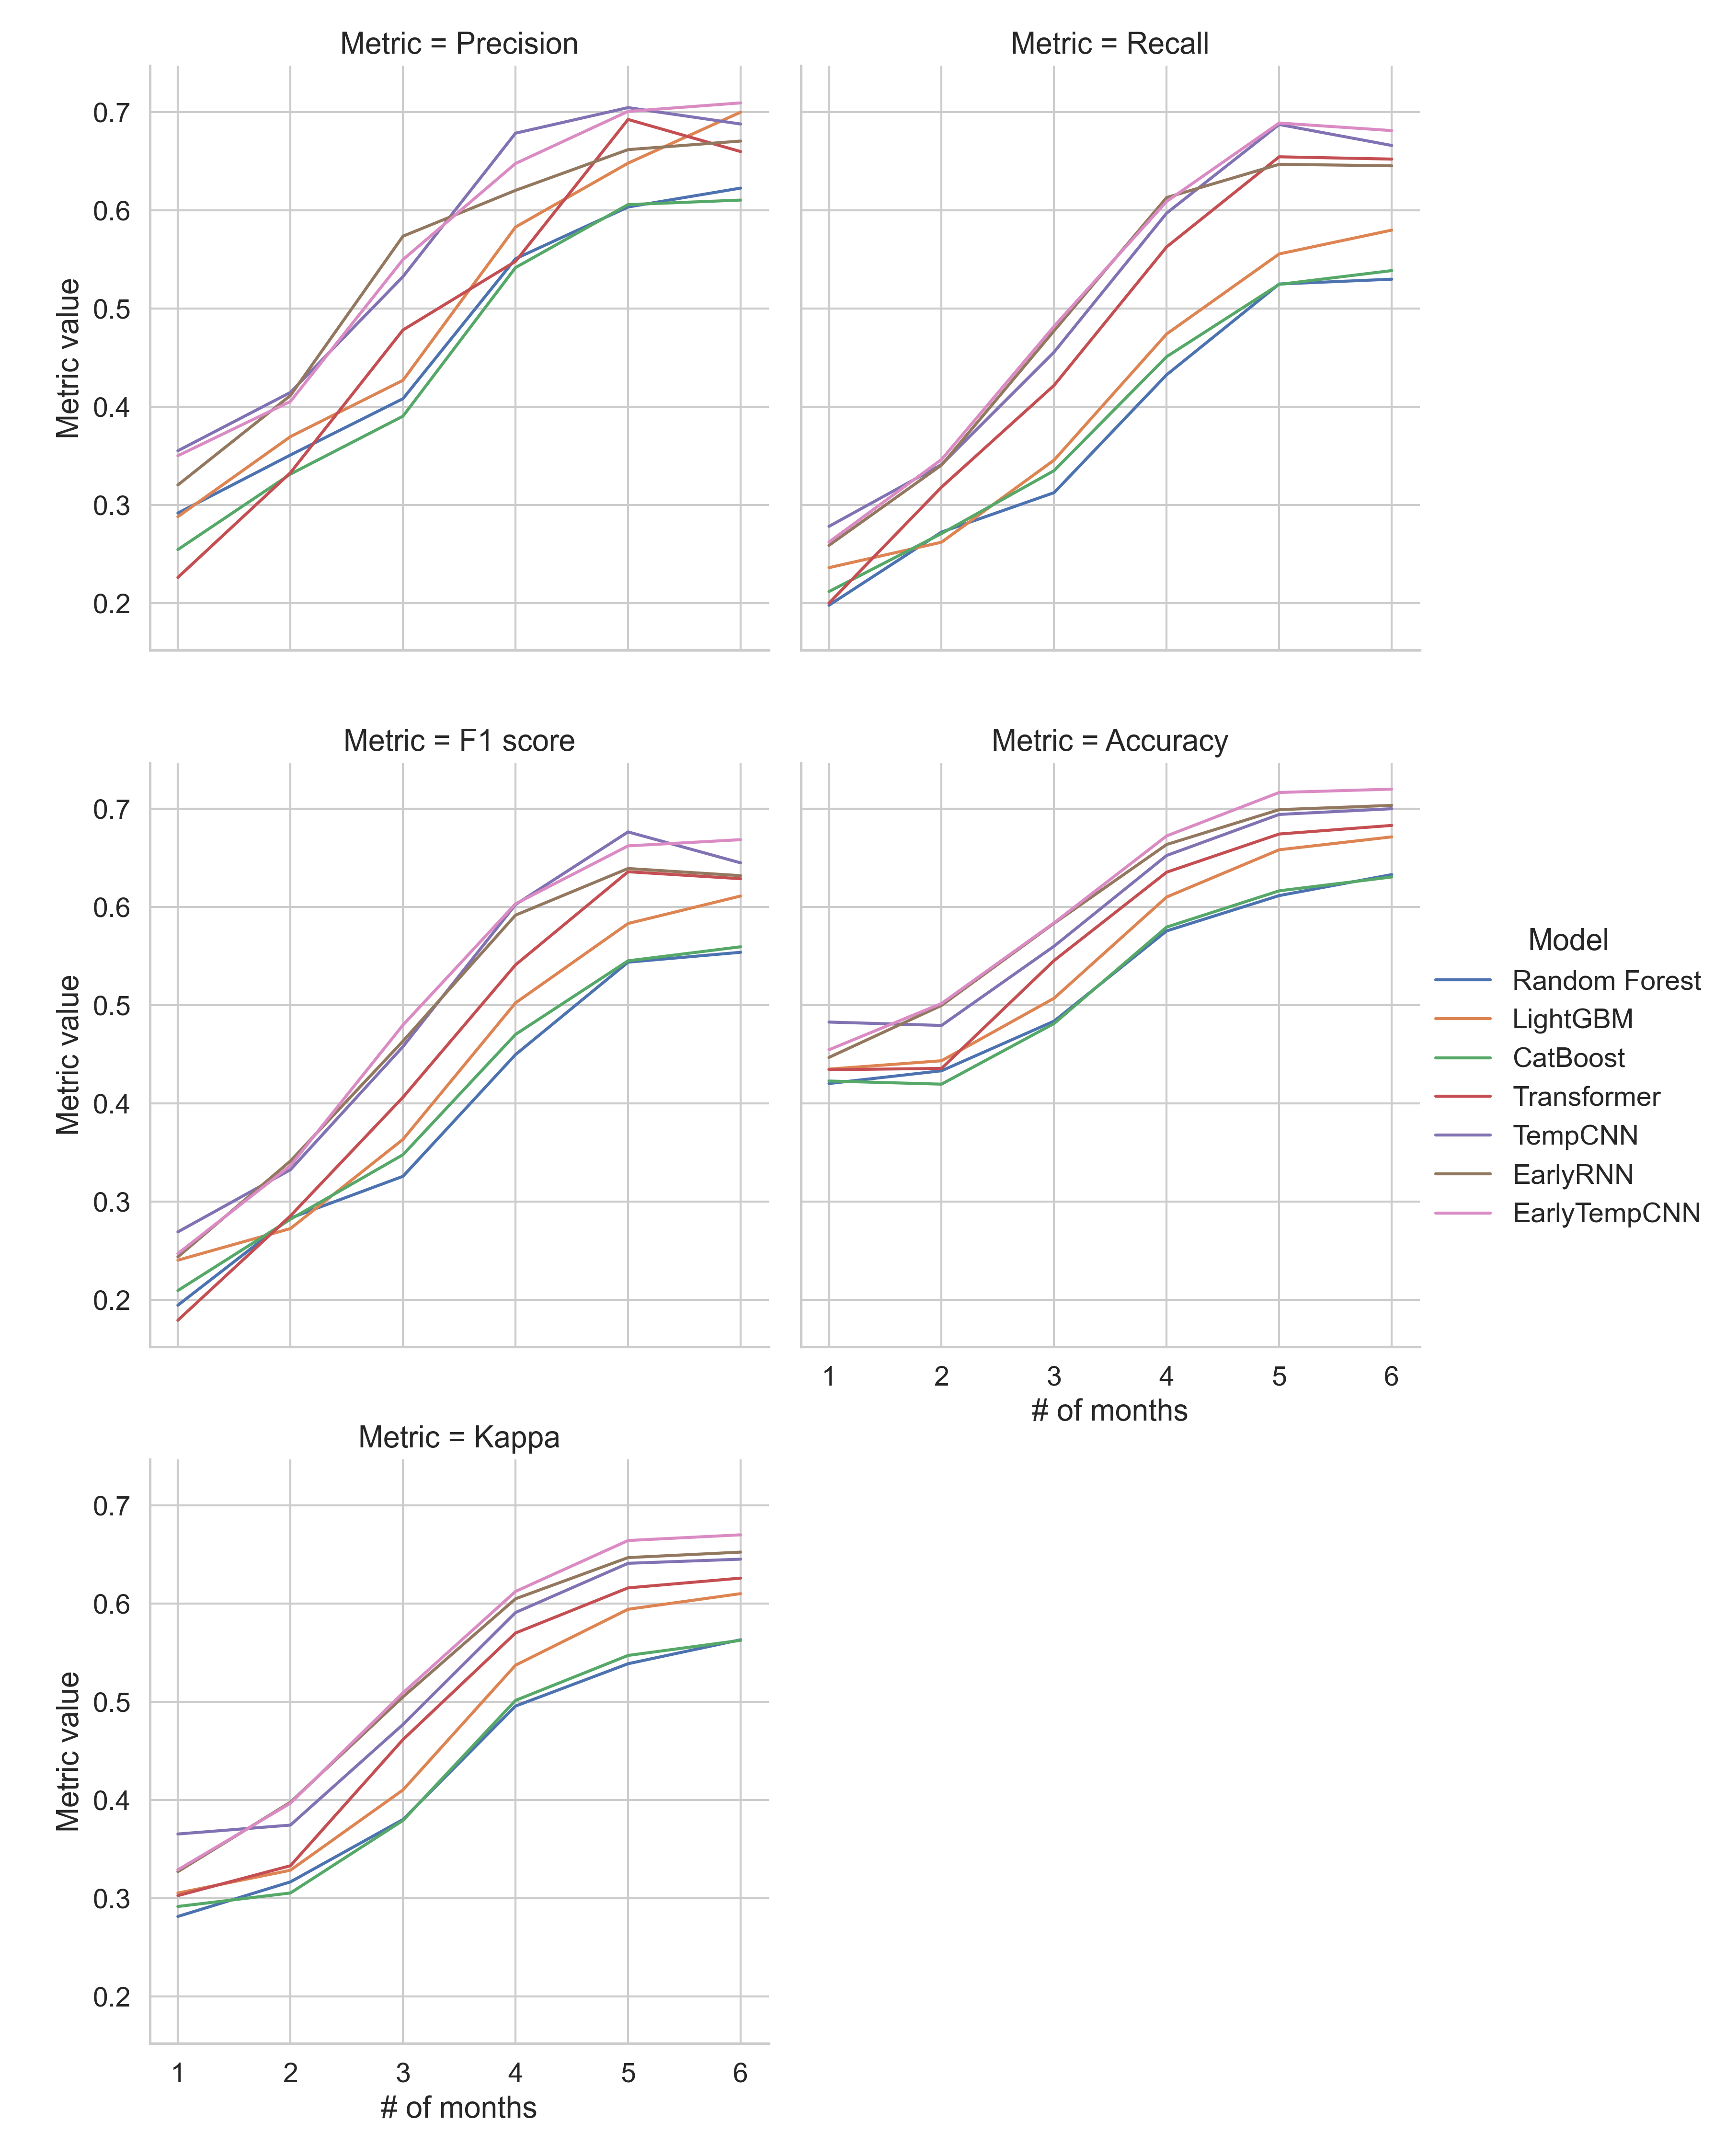
\includegraphics[width=\textwidth]{images/metrics_plot.png}
    \caption{Models Scores With Respect to Number of Months}
    \label{Figure 4.1.1}
\end{figure}

Absolute values of metrics are different. However, all metrics show a similar pattern of change depending on the number of months from the start of the season: at the beginning, the scores are low, then they grow fast until the fourth month, and then the growth becomes slower. The difference between the fifth and the sixth months is negligible. For some models or metrics, the connection between the length of the input sequence and the score is close to the S-shaped curve, for others it looks more or less linear.

Classical models in general underperform. Transformer model and TempCNN show intermediate results. EarlyRNN and EarlyTempCNN are on the top.

In Table \ref{Table 4.1.2}, F1 scores of models depending on the number of months used for classification are represented. This table acts as a supplement to the plot enabling us to look at the precise values of metrics. The top score in each column (i.e. the optimal input length for each model) is given in bold, and the top score in each row (i.e. the best model for the given data length) is italicized. The top scores are reached for input sequences which correspond to five or six months depending on the model. EarlyTempCNN and TempCNN models outperform in most cases, and the top overall  F1 score is reached by TempCNN for the five-month input sequence. 

\begin{table}
\centering
\caption{F1 Scores of Models Depending on the Number of Months}
\label{Table 4.1.2}
\begin{tabular}{lrrrrrrr}
\toprule
model &  catboost &  earlyrnn &  earlytempcnn &  lgbm &    rf &  tempcnn &  transformer \\
n\_months &           &           &               &       &       &          &              \\
\midrule
1        &      0.21 &      0.24 &          0.25 &  0.24 &  0.19 &     \textit{0.27} &         0.18 \\
2        &      0.28 &      \textit{0.34} &          \textit{0.34} &  0.27 &  0.28 &     0.33 &         0.29 \\
3        &      0.35 &      0.46 &         \textit{ 0.48} &  0.36 &  0.33 &     0.46 &         0.41 \\
4        &      0.47 &      0.59 &          \textit{0.60} &  0.50 &  0.45 &     \textit{0.60} &         0.54 \\
5        &      0.55 &      \textbf{0.64} &          0.66 &  0.58 &  0.54 &     \textbf{\textit{0.68}} &         \textbf{0.64} \\
6        &     \textbf{ 0.56} &      0.63 &          \textit{\textbf{0.67}} &  \textbf{0.61} &  \textbf{0.55} &     0.64 &         0.63 \\
\bottomrule
\end{tabular}
\end{table}

\subsection{Earliness \textit{vs} Accuracy}

The main idea of special models (EarlyRNN and EarlyTempCNN) used in the second branch of experiments is to find a trade-off between earliness and accuracy. According to the previous section, it is clear that such models reach performance comparable to generic models. However, as it was mentioned in the implementation notes, there is no direct way to compare the performance of generic models with the performance of specific models, because they achieve the earliness of prediction by different means (to be precise, “earliness” of generic models is just a reduction of the amount of data which is being provided to them). Consequently, the results in the previous section end up being a form of “pseudo-comparison”. Nevertheless, it is still possible to look at the “natural” performance of special models.

The output of special models consists of two parts. The first one is a tensor of dimension $T \times C$, where $T$ is the length of the input time series and $C$ is the number of classes, containing log probabilities of each class for a given timestamp. The second one is a one-dimensional tensor of length $T$ containing the probability of stopping at this time point. When the probability is high enough, it means that the model is confident in its prediction, and so no more data is necessary, and the predicted label at this time point may be output as a final prediction. The time point where probability has become high enough is called a stopping point. The stopping point for each field is different. For example, for one field a classification may be done using only the first 10 elements of the input sequence, while for another 20 or 30 may be required. Taking into account this algorithm for making the final prediction, we may calculate two metrics: (1) the dataset-average score at the stopping point and (2) the dataset-average stopping time.

In Figures \ref{Figure 4.2.1} and \ref{Figure 4.2.2}, F1 scores of two special models and average stopping times are shown. It may be seen that during the training, both models quickly reach results comparable to generic models utilizing slightly less than $2/3$ of the time series (according to my implementation, 35–40 time points correspond to 3.5–4 months, because each month is represented as 10 time points).


\begin{figure}
    \centering
    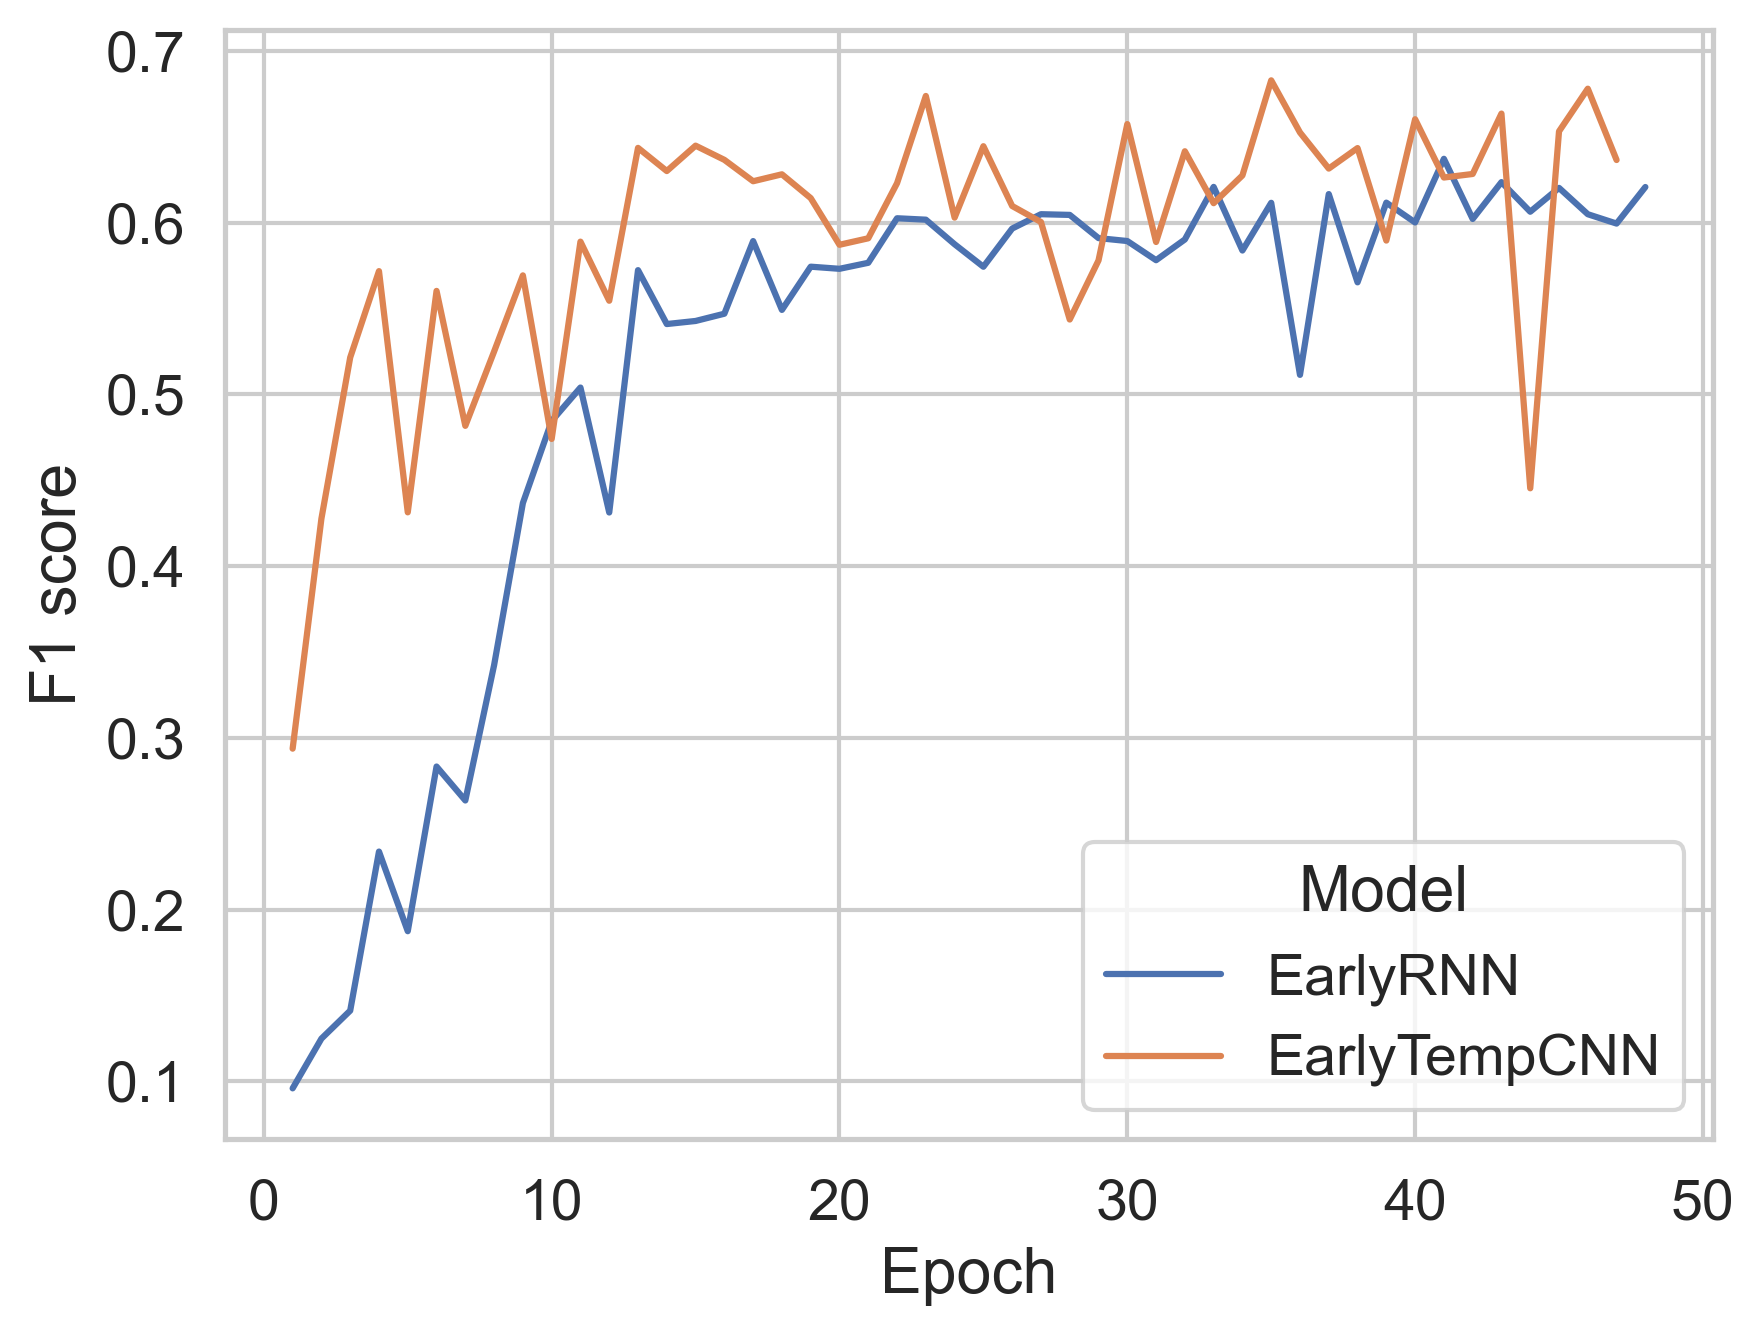
\includegraphics[width=\textwidth]{images/early_fscores.png}
    \caption{Dataset-Average F1 Scores of EarlyRNN and EarlyTempCNN Models}
    \label{Figure 4.2.1}
\end{figure}

\begin{figure}
    \centering
    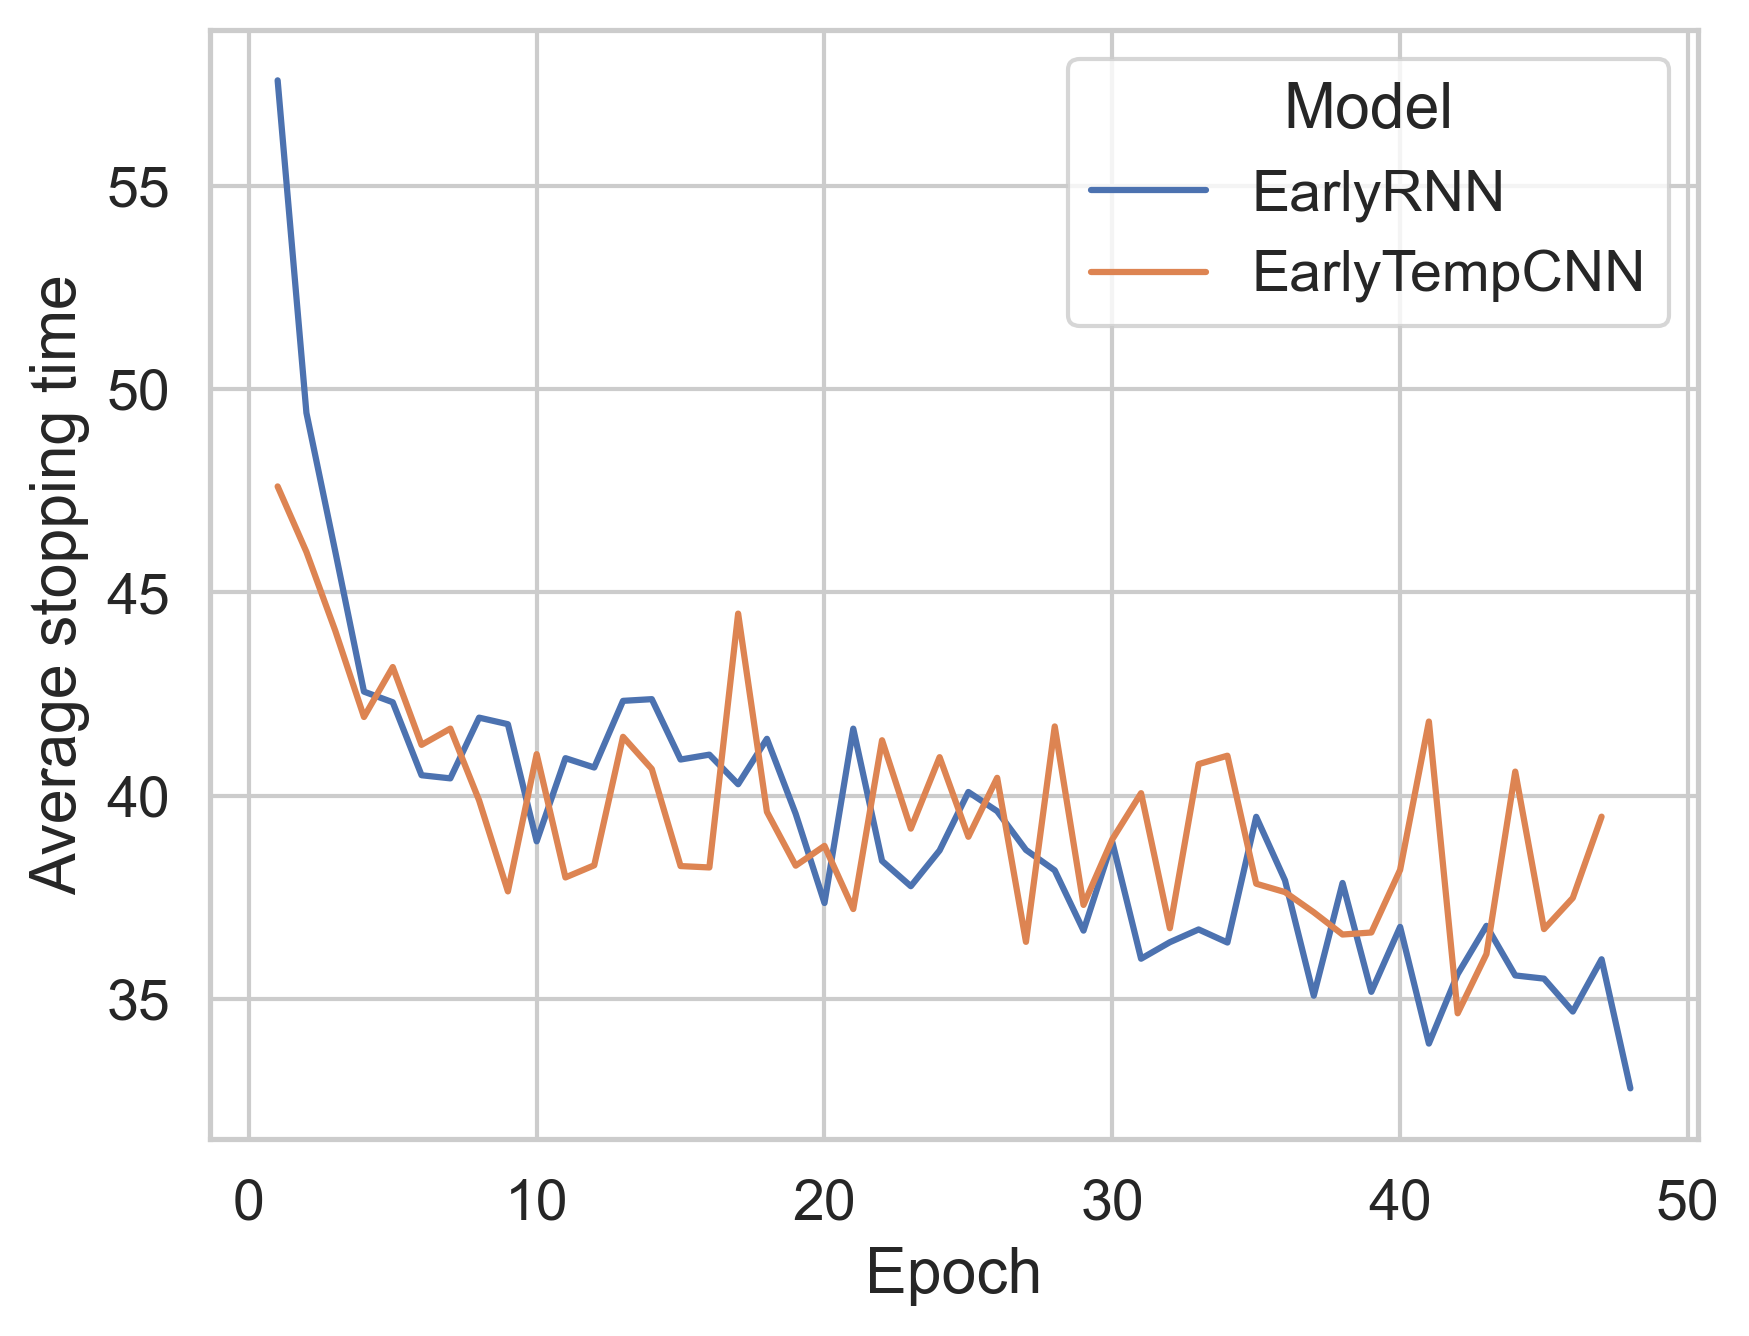
\includegraphics[width=\textwidth]{images/early_stopping_time.png}
    \caption{Dataset-Average Stopping Time of EarlyRNN and EarlyTempCNN Models}
    \label{Figure 4.2.2}
\end{figure}

\subsection{Single-Field Inference}

All models used in this research can predict crop classes based on full-length or limited-length input time series. The exact algorithm is different for generic models and for special models. For generic models, we have to get subsamples of input data having the required length $T$ and feed them into the separate models which were pre-trained on the subsamples of the same length. For special model, we can take a time series of any length and directly get the class probabilities and the probability of stopping.


\begin{figure}
    \centering
    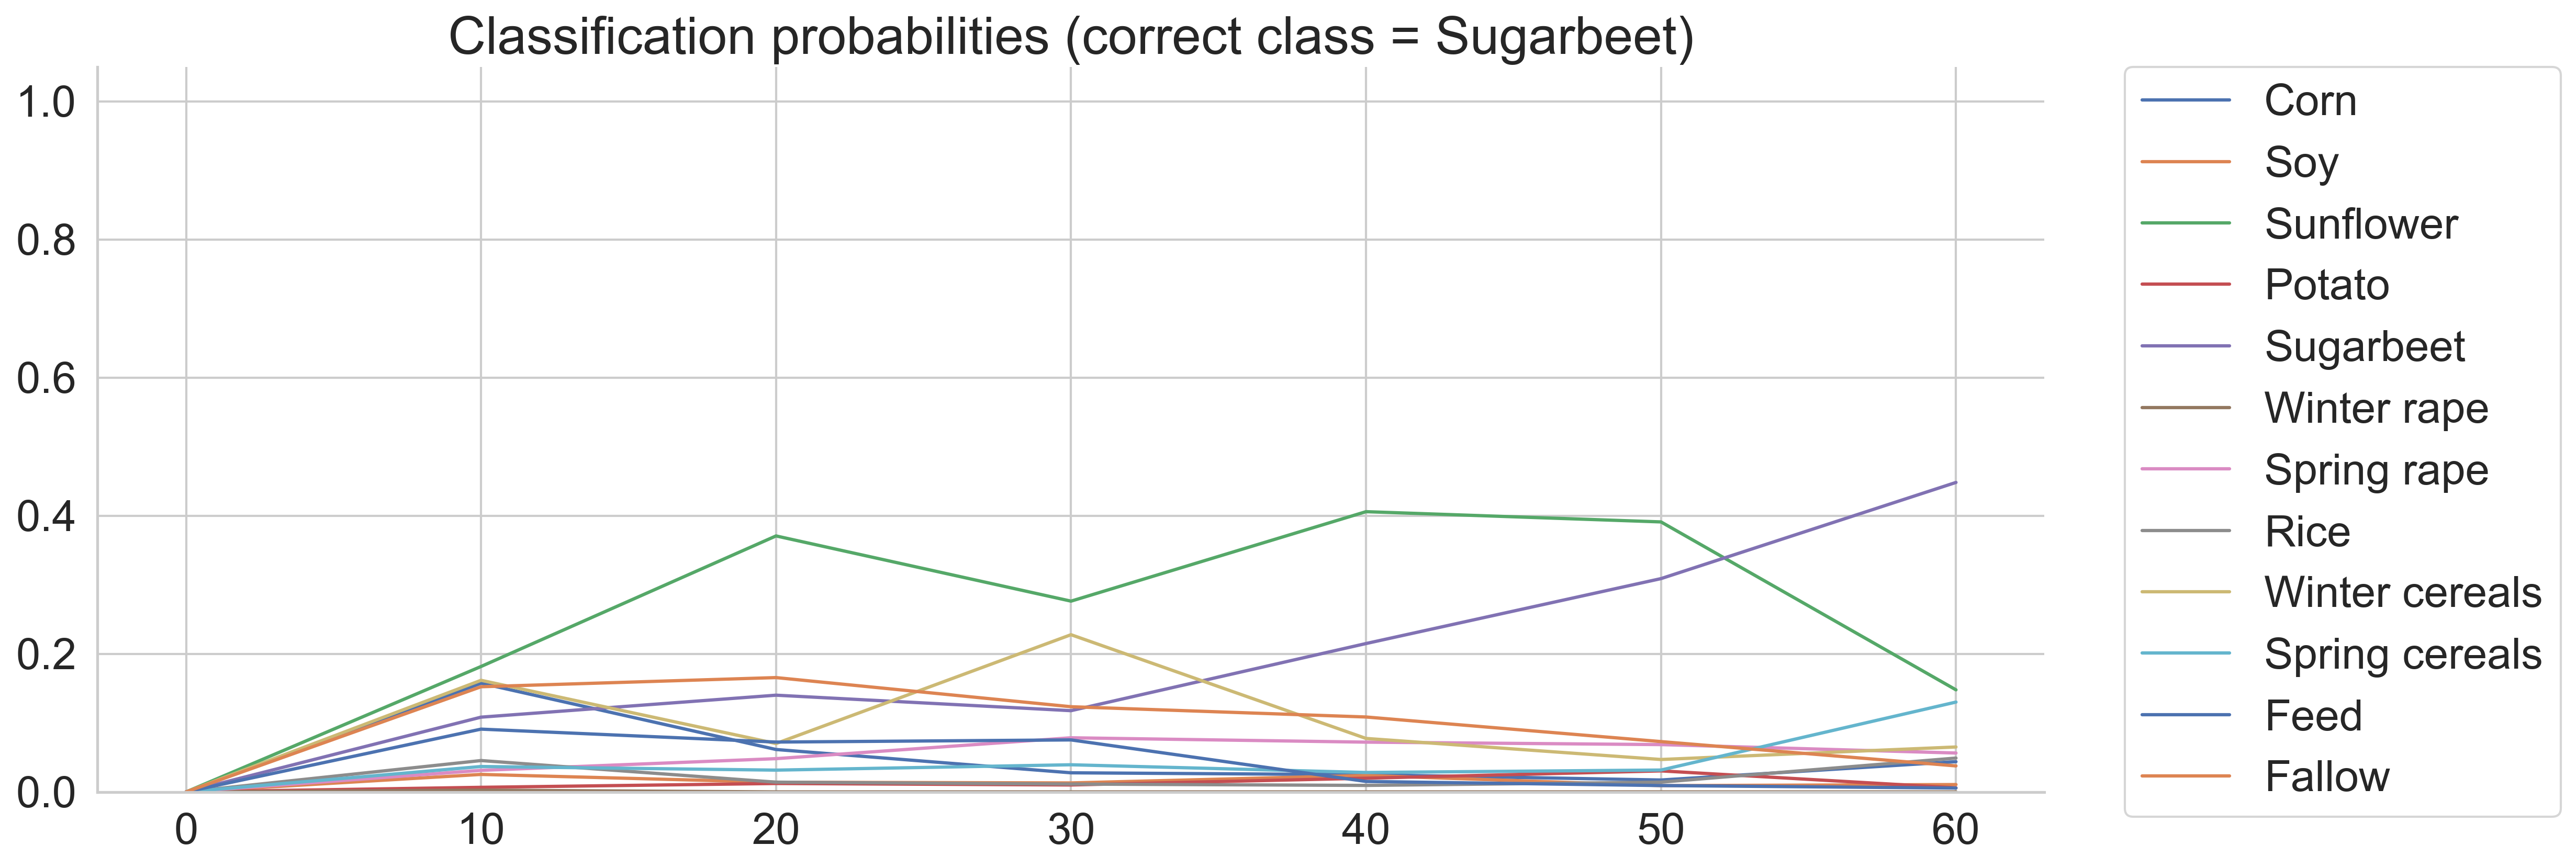
\includegraphics[width=\textwidth]{images/rf_preds.png}
    \caption{Single-Field Prediction of Random Forest Ensemble}
    \label{Figure 4.3.1}
\end{figure}


\begin{figure}
    \centering
    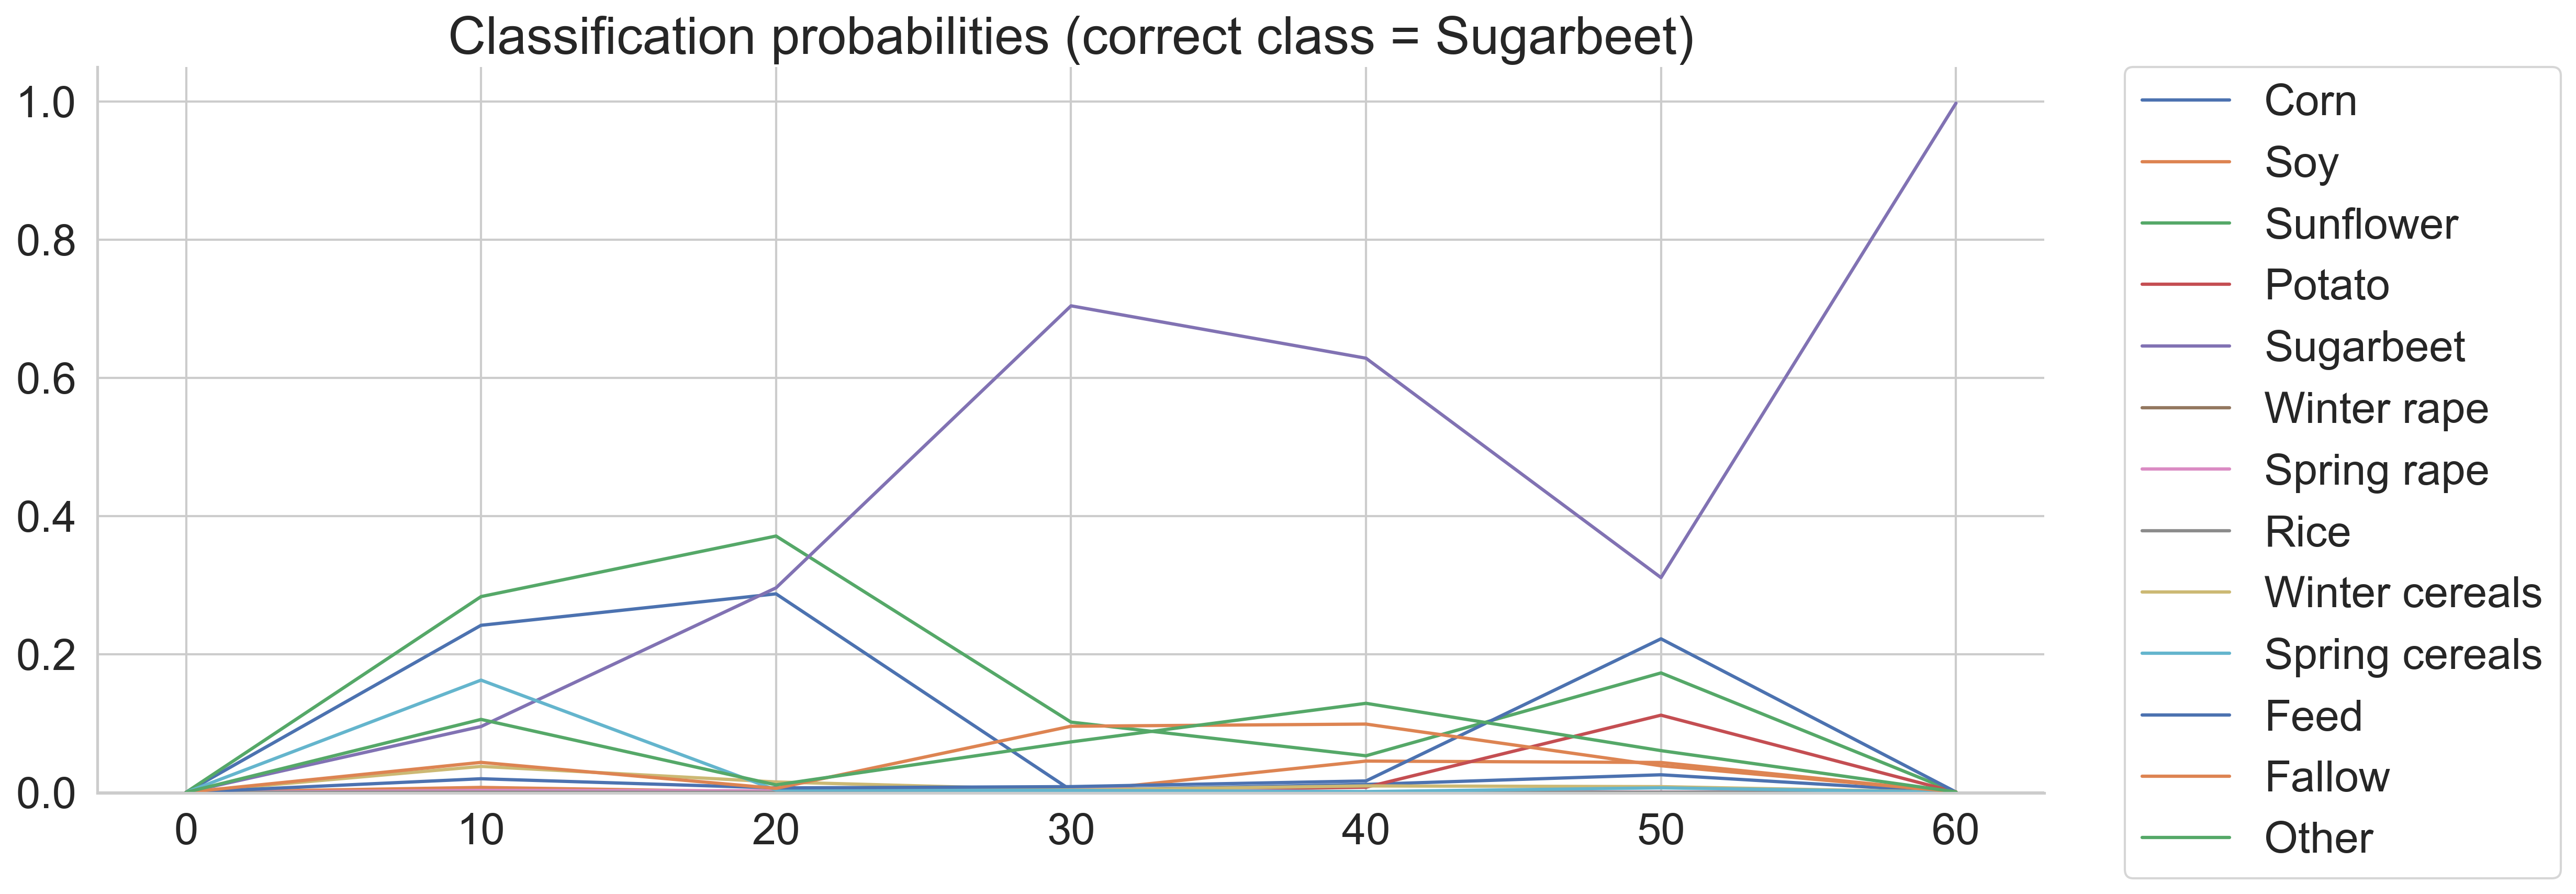
\includegraphics[width=\textwidth]{images/tempcnn_preds.png}
    \caption{Single-Field Prediction of TempCNN Ensemble}
    \label{Figure 4.3.2}
\end{figure}


\begin{figure}
    \centering
    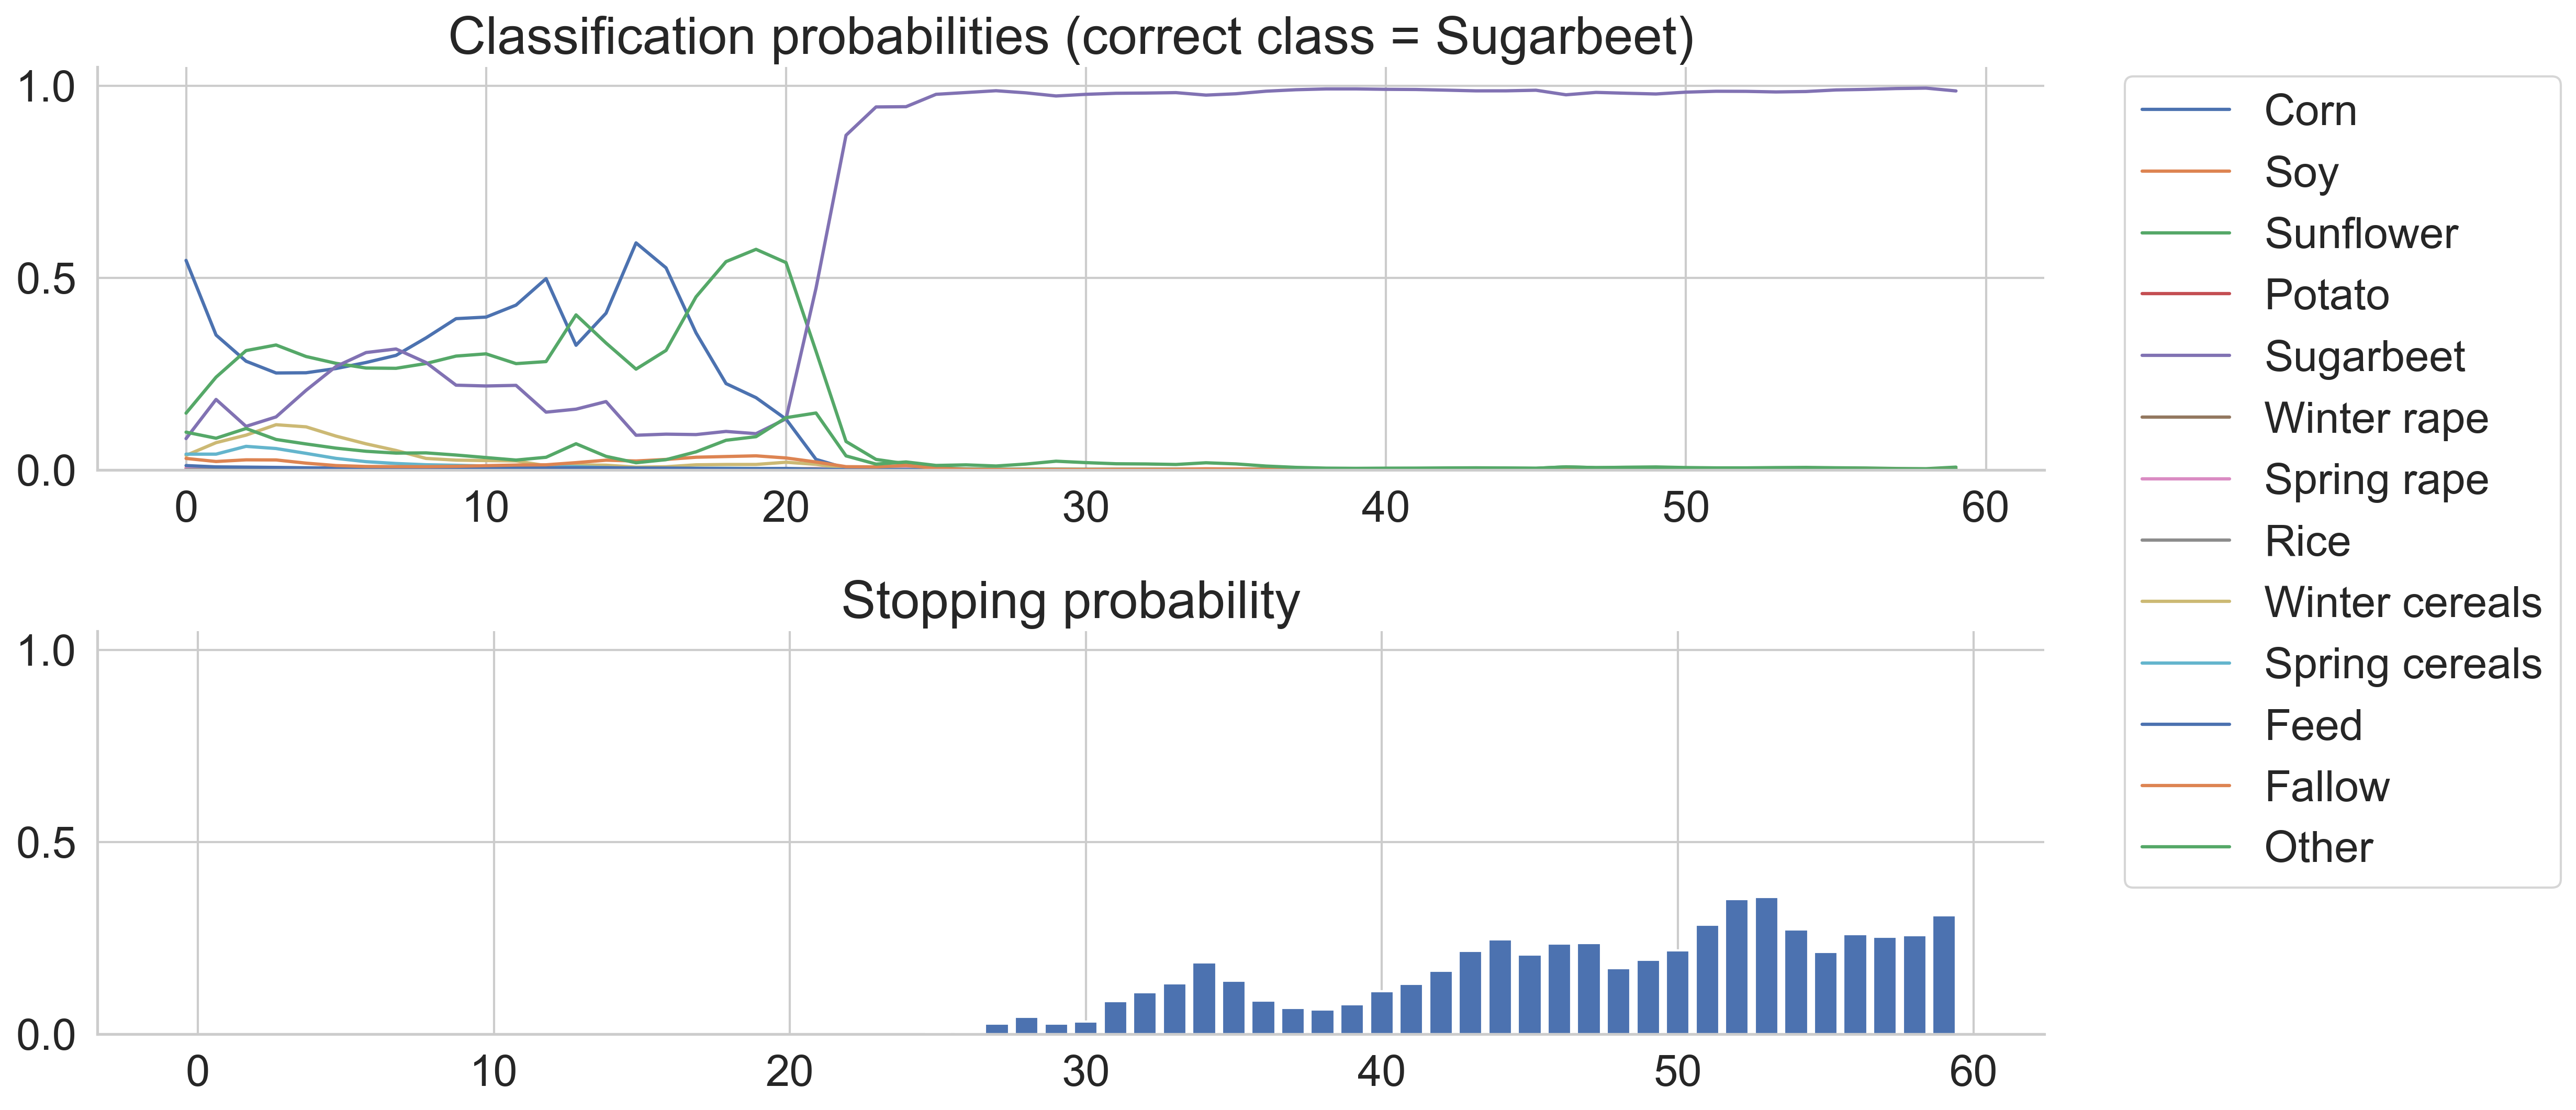
\includegraphics[width=\textwidth]{images/earlyrnn_preds.png}
    \caption{Single-Field Prediction of EarlyRNN}
    \label{Figure 4.3.3}
\end{figure}


\begin{figure}
    \centering
    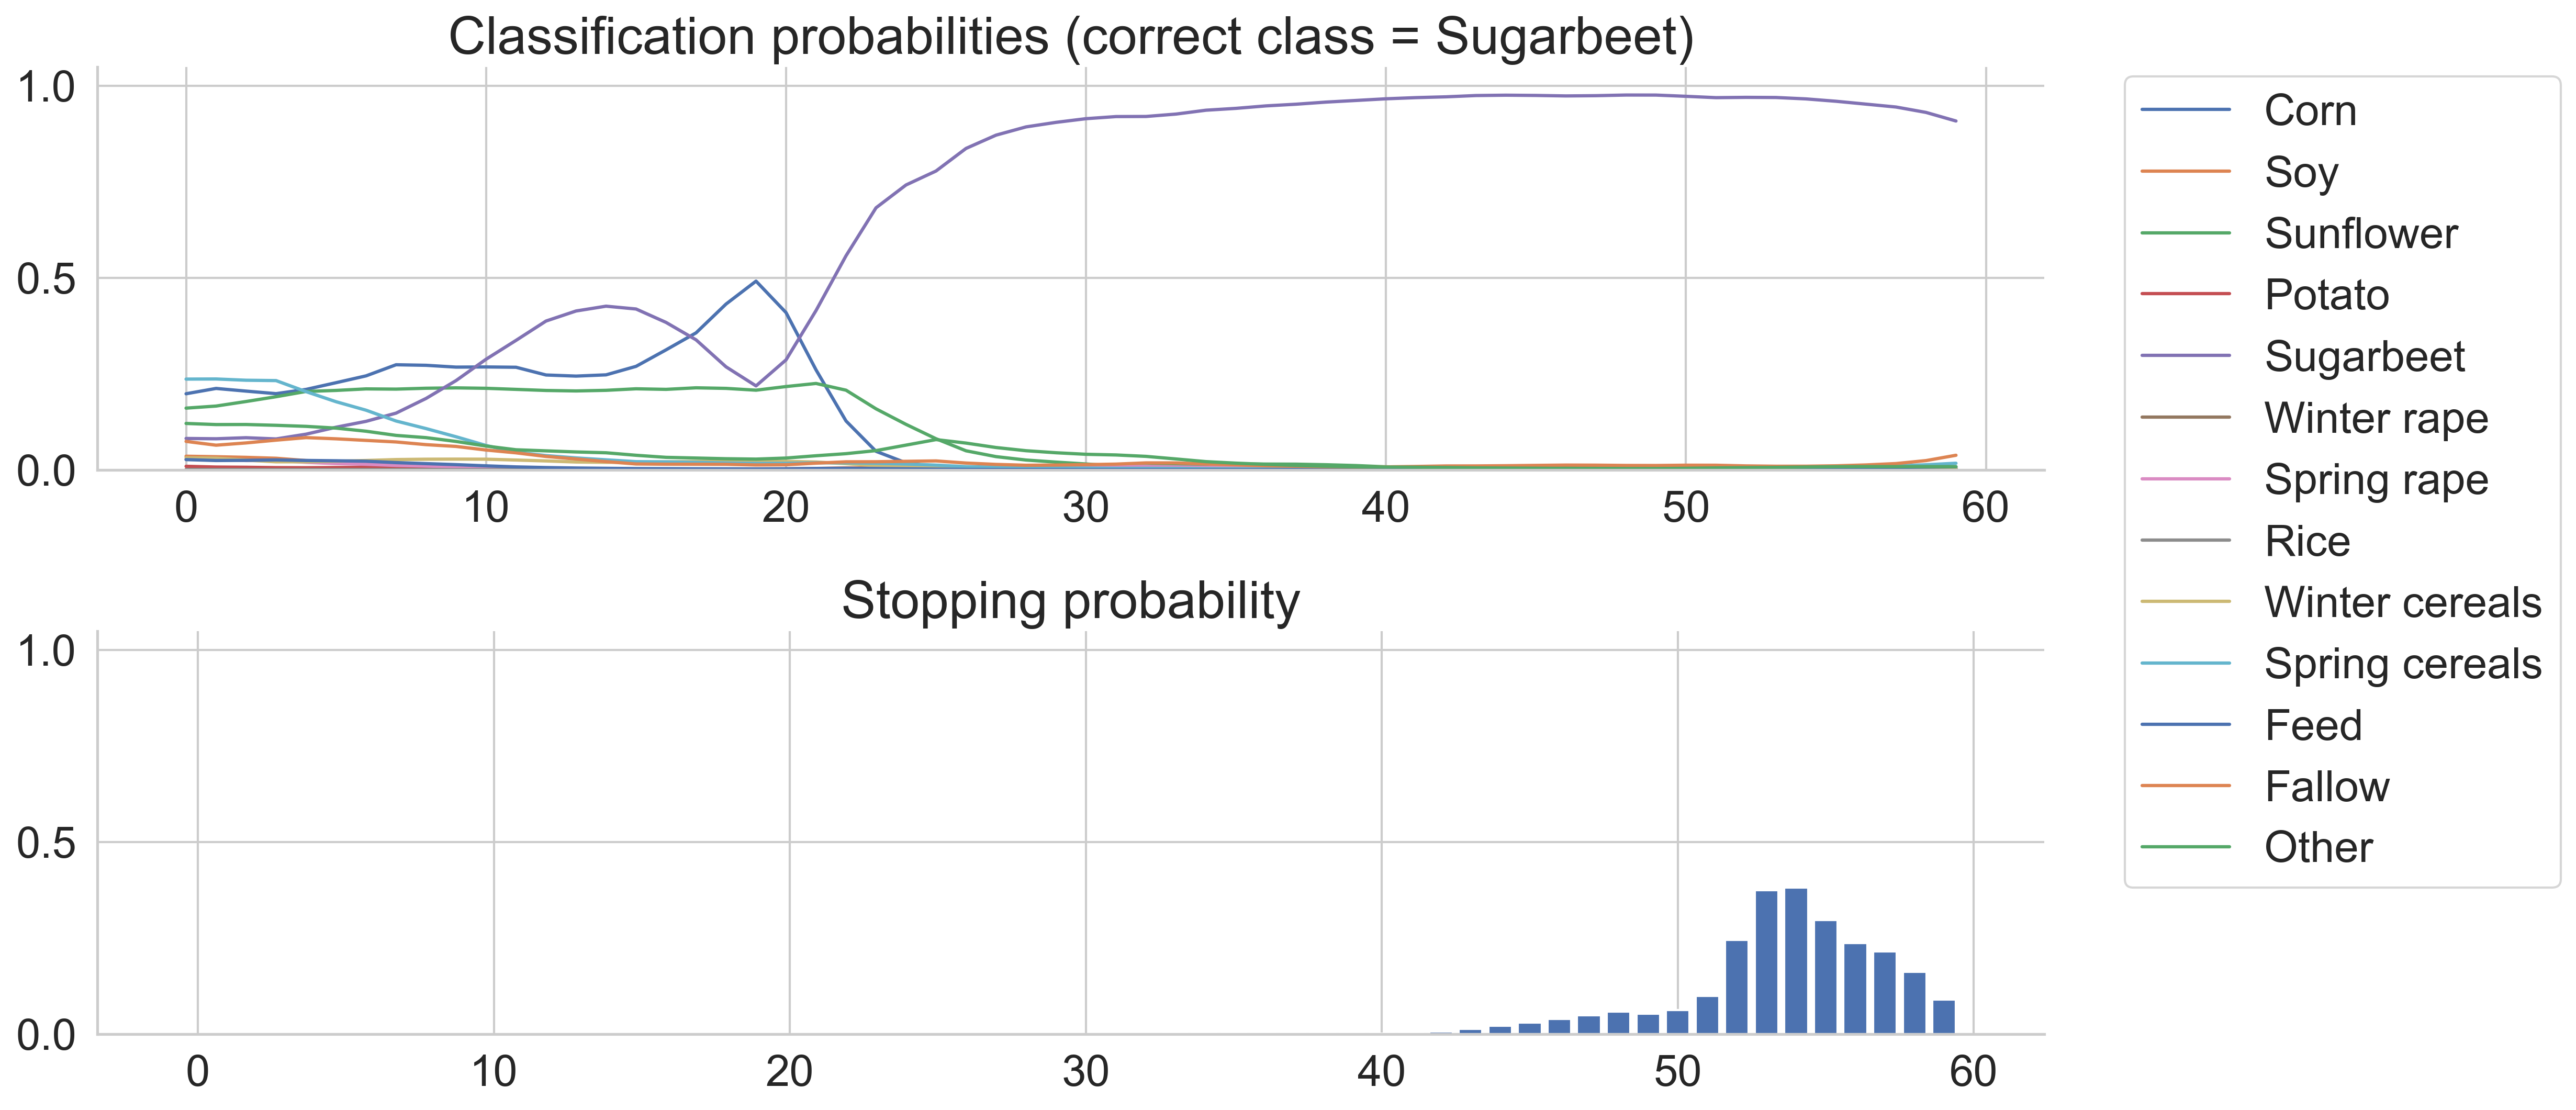
\includegraphics[width=\textwidth]{images/earlytempcnn_preds.png}
    \caption{Single-Field Prediction of EarlyTempCNN}
    \label{Figure 4.3.4}
\end{figure}

In Figures \ref{Figure 4.3.1}, \ref{Figure 4.3.2}, \ref{Figure 4.3.3}, \ref{Figure 4.3.4}, the temporal change of class probabilities predicted by four models for field \#10 of the test part of the dataset is shown. For EarlyRNN and EarlyTempCNN, the stopping probability is also plotted. It is clear that at the beginning of the season, the probabilities of all classes are almost equal and low, and the probability of an incorrect class is sometimes higher than the probability of a correct class. By using more data, a model learns to make better predictions. At some time point, the probability of the correct class grows and becomes the largest. For EarlyRNN and EarlyTempCNN, this correct distribution of probabilities then does not change. An ensemble of Random Forest models begins to classify the field correctly only by the end of the season. An ensemble of TempCNN models returns correct crop label very early, but by the end of the season, there is a risk of getting a wrong answer (at least with a given field). For special models, the stopping probability is zero at the first part of the season, and after that starts increasing. Note that the increase in stopping probability is accompanied by the rise of correct class probability, but with a substantial lag.

\subsection{Robustness Check}

For a robustness check, the models were re-trained on the data of the year 2021. Tree-based models hyperparameters and neural-based models training settings were the same as in the main flow of the experiments. The metrics plot similar to the plot of 2018's main results and the table of F1 scores (Figure \ref{Figure 4.4.1} and Table \ref{Table 4.4.1}, respectively) are shown below. The scores have increased by approximately 0.1. The dependence between input time series length and the scores still exists and is close to the S-shaped logistic curve in most of the cases. Also, the scores for six, five and four months are nearly the same. That is in contrast with the results of the main experiments, where dropping last two months of input data resulted in a greater decline in performance. As for individual models, here it is Transfromer and TempCNN that achieve the top scores. At the same time, EarlyRNN and EarlyTempCNN underperform, and their results are among the lowest. Traditional tree-based Random Forest and Catboost also show low results, while LightGBM is somewhere in the middle.


\begin{figure}
    \centering
    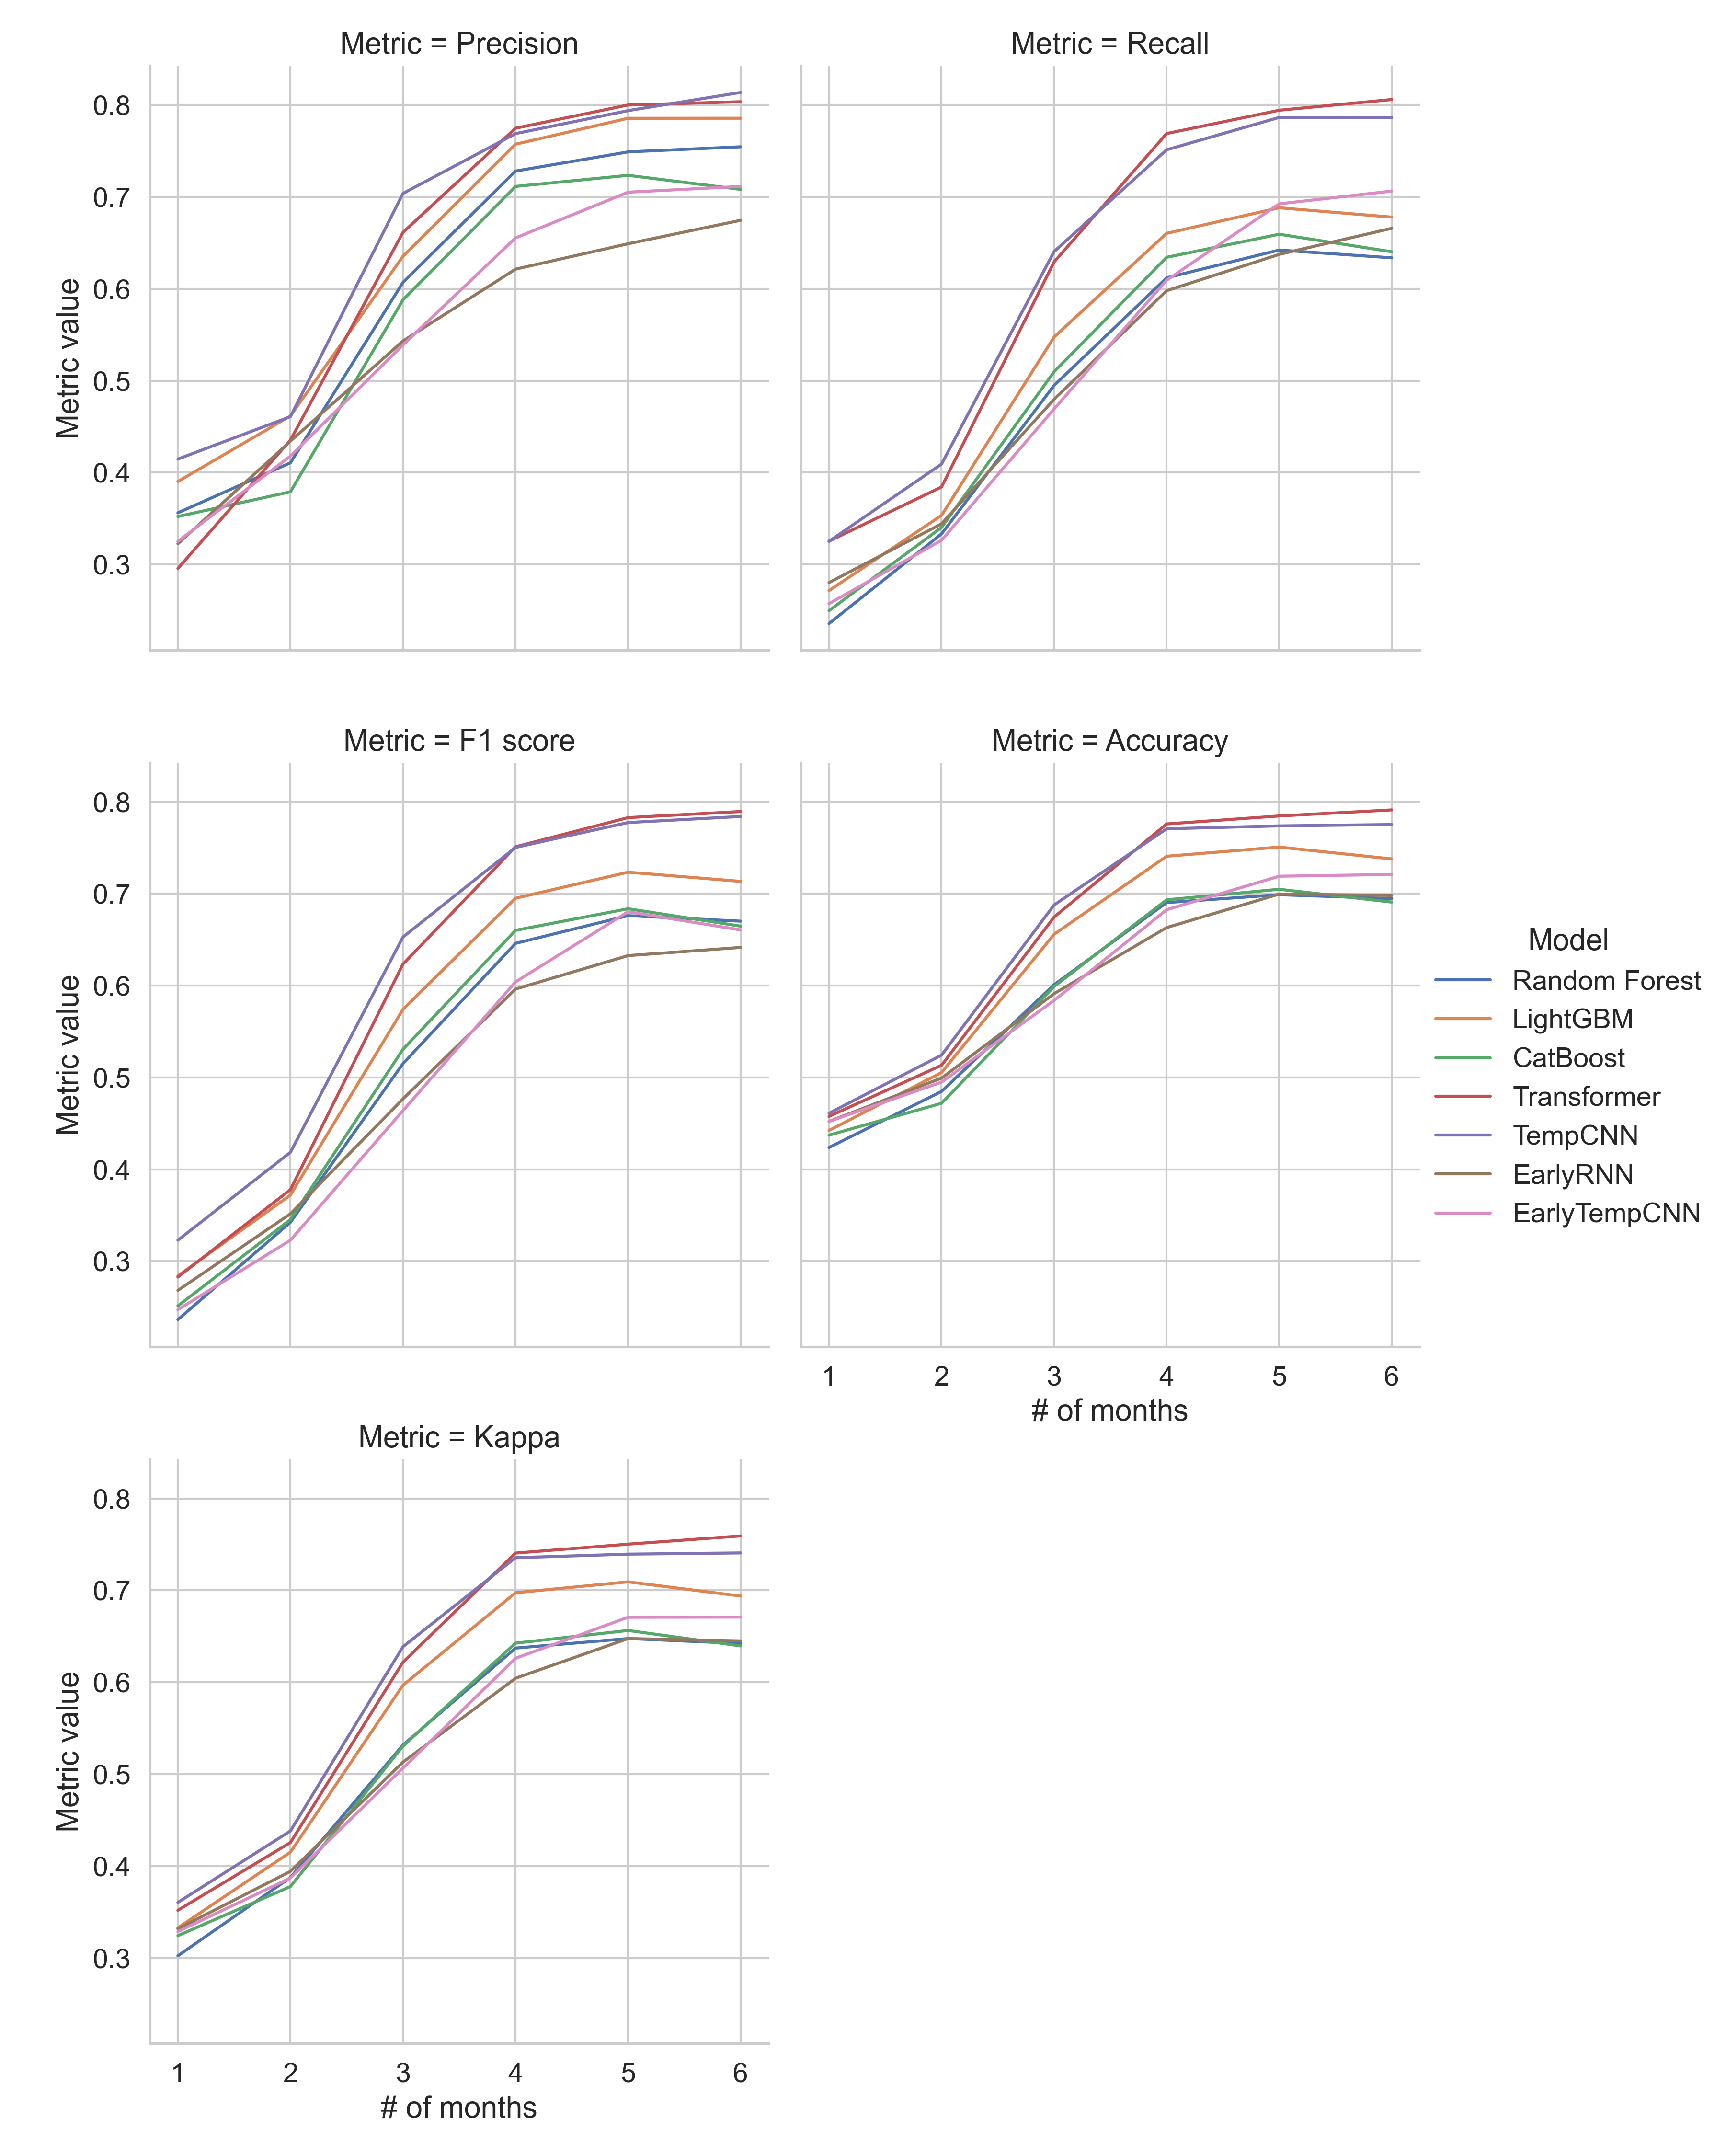
\includegraphics[width=\textwidth]{images/metrics_plot_2021.png}
    \caption{Models Scores With Respect to Number of Months}
    \label{Figure 4.4.1}
\end{figure}


\begin{table}
\centering
\caption{F1 Scores of Models Depending on the Number of Months Based on 2021 Data}
\label{Table 4.4.1}
\begin{tabular}{lrrrrrrr}
\toprule
model &  catboost &  earlyrnn &  earlytempcnn &  lgbm &    rf &  tempcnn &  transformer \\
n\_months &           &           &               &       &       &          &              \\
\midrule
1        &      0.25 &      0.27 &          0.25 &  0.28 &  0.24 &     \textit{0.32} &         0.28 \\
2        &      0.35 &      0.35 &          0.32 &  0.37 &  0.34 &     \textit{0.42} &         0.38 \\
3        &      0.53 &      0.48 &          0.46 &  0.57 &  0.52 &     \textit{0.65} &         0.62 \\
4        &      0.66 &      0.60 &          0.60 &  0.70 &  0.65 &     \textit{0.75} &         \textit{0.75} \\
5        &      \textbf{0.68} &      0.63 &          \textbf{0.68} &  \textbf{0.72} &  \textbf{0.68} &     \textbf{\textit{0.78}} &         \textit{0.78} \\
6        &      0.66 &      \textbf{0.64} &          0.66 &  0.71 &  0.67 &    \textbf{ 0.78} &         \textbf{\textit{0.79}} \\
\bottomrule
\end{tabular}
\end{table}

\section{Discussion}

The results of my research show that all the models trained for the experiments have similar performance. Classical machine learning methods like tree-based ensembles are slightly worse, while novel convolutional, recurrent, and attention-based neural networks have better scores. All the scores obtained on the dataset used for this study are lower that the scores from reference papers. The possible explanations include a limited amount of training data, a class imbalance, a relatively big number of classes, and wide geographical range of fields. However, the results of my study are in line with the general tendency observed in the literature that neural networks outperform classical machine learning methods for the task of crop classification based on time series of remote sensing data.

All the models are sensitive to the length of input data sequences, that is, the smaller part of the season is used, the less accurate the predictions are. However, the decline in the quality of the classification using only four months of the season out of six is considerably small. Thus, it may be concluded that all the models can give good predictions utilizing only $2/3$ of seasonal data. In practical terms, it means that if a season starts in April, an accurate enough classification may be obtained by the end of July. Also, the predictions using only five months out of six are almost the same as the predictions on the full-length data, thus the last month of the season is nearly useless for the predictions and may be dropped freely, reducing the amount of necessary data by $1/6$.

The performance of special models optimized jointly for earliness and accuracy, if measured at the same monthly intervals as the performance of generic models, is almost equal to the performance of regular neural-based models. However, they have at least three important advantages. First, they are trained in one turn, whereas using regular models, it is necessary to train an ensemble of several models, increasing the costs of computations. Next, on average their scores are very close to the scores of regular models using full-length data, but to reach such scores, they require only about $2/3$ of the initial data sequence. Last, these models produce class probabilities and probability of stopping for each time point and for each field individually, thus allowing for more fine-tuned field-based applications, e.g. getting real-time input data flow for the current season from ongoing satellite observations, classifying each field separately, detecting model's confidence and providing the final result as early as possible once the target confidence is reached.

The overall positive curvilinear connection between the length of input time series used for the classification and the performance of the models is supported by the results of re-training the models using the year 2021 data. Besides, the S-shaped nature of this relationship has become more visible and clear. From the results obtained from year 2021 data it can be concluded that the difference in the quality of models which use four, five, or six months of the season is very small, and in most cases, four-month data is enough for as accurate a classification as obtained on full-length data. In other words, while in 2018 only the last month of the season may have been dropped without any substantial loss in the scores, in 2021, probably thanks to the larger dataset size, the last two months of the season may be omitted without any significant reduction in quality. So, perhaps the size of the training dataset is also important for the earliness. 

It is worth mentioning that the increase in the size of the training dataset combined with the change of year has led to notable growth in overall performance. For example, the scores of top models have reached the state-of-the-art scores reported in relevant papers. However, not every result of the main experiments is reproduced during the robustness check. Special models (EarlyRNN and EarlyTempCNN) here have acted relatively poorly and have been comparable to baseline tree-based solutions only, thus maybe the advantages of such models are more expressed on small datasets, while on larger datasets, the ensembles of state-of-the-art neural networks outperform. Nevertheless, it is interesting that the proposed EarlyTempCNN still acts a bit better than EarlyRNN.

\section{Conclusion}

\begin{enumerate}
    \item It is possible to classify crops correctly enough using satellite observations data with a time range from April to the beginning of August only. There is a slight reduction in performance, but it is relatively small and tolerable in most of the applications. The last month of the season (September) may be dropped from input data practically without any loss in quality. If a large training dataset is used, the last two months of the input time series (August and September) may be dropped without any effect on quality.
    \item Neural-based models are in general of better performance than tree-based models.
    \item Special models designed for simultaneous optimization of earliness and accuracy act as well as ensembles of traditional tree-based models, but provide additional benefits like reduction in training time, field-tailored predictions, and real-time confidence estimates. The results of their comparison with more modern neural-based models are mixed. It is likely that on small training datasets special models are better than generic ones, while if the dataset is large, an ensemble of generic models trained on varied-length input sequences is better.
    \item A proposed EarlyTempCNN model slightly outperforms the original EarlyRNN model it is based on.
\end{enumerate}

\newpage

\printbibliography


\end{document}
